\begin{frame}{Algorithm overview}
    \begin{itemize}
        \item \textbf{ProbCons\cite{do2005probcons}} is a pair-hidden Markov model-based progressive alignment algorithm that differs from most typical approaches in its use of \textbf{maximum expected accuracy} rather than Viterbi alignment, and of the probabilistic consistency transformation to incorporate multiple sequence conservation information during pairwise alignment. 
        \item \textbf{Hidden Markov Models (HMMs)} in sequence analysis are based on a strong probabilistic model that \textbf{includes a representation of INDELs} (insertions and deletions, i.e. gaps). 
        \item The HMM describing families of related sequences are called \textbf{profile HMMs}
    \end{itemize}
\end{frame}

\begin{frame}{Algorithm overview}
    \begin{itemize}
        \item In profile HMMs the residues in each position of the alignment can be in one of three possible states:
        \begin{enumerate}
            \item \textbf{Match:} represent conserved position
            \item \textbf{Insert:} represent small stretches of nonspecific sequence
            \item \textbf{Delete:} correspond to gaps and represent the absence of a conserved residue
        \end{enumerate}
        \item Each state has associated:
        \begin{enumerate}
            \item \textbf{Emission probability:} correspond to the probability of observing each amino acid at that particular position of the alignment
            \item \textbf{Transition probability:} describes the frequency of observing a match, insertion or deletion in column i+1 given the state column i. 
        \end{enumerate}
    \end{itemize}
    
\end{frame}

\begin{frame}{Algorithm overview}
\centering
 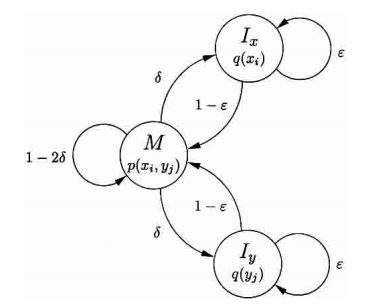
\includegraphics[width=0.35\linewidth]{img/hmm_states.PNG}
 \begin{itemize}
     \item Emission probabilities, which correspond to traditional substitution scores, are based on the BLOSUM62 matrix.
     \item Transition probabilities, which correspond to gap penalties, are trained with unsupervised Expectation-Maximization (EM)
     \begin{itemize}
         \item $\pi_{insert}$: initial insertion probability parameter
         \item $\delta$: insertion start probability parameter
         \item $\epsilon$: insertion extension probability parameter
     \end{itemize}
     \item The resulting parameters ($\delta$ = 0.019931, $\epsilon$ = 0.79433, $\pi_{insert}$= 0.19598) are used as the default for the program.

 \end{itemize}
    
\end{frame}

\begin{frame}
    \frametitle{Algorithm overview}

    \begin{block}{ProbCons \cite{do2005probcons}}
        \begin{itemize}
            \item Given $m$ sequences $\rightarrow$ $S = \{s^{(1)}, \ldots, s^{(m)} \}$.
            \item Maximum expected accuracy.
            \item Probabilistic consistency $\rightarrow$ MSA conservation information in the pairwise alignment.
        \end{itemize}
    \end{block}
    
    \begin{enumerate}
        \item Step 1: Computation of posterior probability matrices.
        \item Step 2: Computation of expected accuracies.
        \item Step 3: Probabilistic consistency transformation.
        \item Step 4: Computation of the guide tree.
        \item Step 5: Progressive alignment.
        \item Step 6: Iterative refinement (post-processing OPTIONAL step).
    \end{enumerate}
\end{frame}

\begin{frame}
    \frametitle{Step 1: Computation of posterior probability matrices}
    \begin{itemize}
        \item For $x, y \in S$, compute the matrix
        \begin{align*}
            P_{xy}(i,j) = \pmb{P}(x_i \sim y_j \in a^* | x, y) \;,
        \end{align*}
        where $1\leq i\leq|x|$ and $1\leq j\leq |y|$.
        \item Each position $P_{xy}(i,j)$ is the \textbf{posterior} probability that letters $x_i$ and $y_j$ are paired i an alignment $a^*$.
        \begin{itemize}
            \item Computing posterior probabilities in pair-HMMs \cite{durbin1998biological}.
        \end{itemize}
        \item Time complexity $O(m^2 L^2)$.
        \begin{itemize}
            \item $m$ is the number of sequences.
            \item $L$ is the length of each sequence.
        \end{itemize}
    \end{itemize}
\end{frame}

\begin{frame}
    \frametitle{Step 2: Computation of expected accuracies}
    \begin{itemize}
        \item The expected accuracy is defined as
        \begin{align*}
            \pmb{E}_{a^*} (acc(a,a^*)|x,y) = \frac{1}{\min{\{|x|,|y|\}}} \sum_{x_i\sim y_j \in a} P_{xy}(i,j) \;,
        \end{align*}
        where $a$ is the align*ment that maximizes the expected accuracy by dynamic programming.
        \item Set 
        \begin{align}\label{eq:score}
            E(x,y) = \pmb{E}_{a^*} (acc(a,a^*)|x,y) \;.
        \end{align}
    \end{itemize}
\end{frame}

\begin{frame}
    \frametitle{Step 3: Probabilistic consistency transformation}
    \begin{itemize}
        \item Reestimate quality scores $\pmb{P}_{xy}$ $\rightarrow$ probabilistic consistency transformation.
        \item Incorporate similarity of $x$ and $y$ to other sequences in $S$:
        \begin{align*}
            {\pmb{P}}'(x_i \sim y_j \in a^* | x, y) = \frac{1}{|S|} \sum_{z\in S} \sum_{z_k \in z} F(x_i, y_j, z_k) \;,
        \end{align*}
        where $F(x_i, y_j, z_k) =  {\pmb{P}}(x_i \sim z_k \in a^* | x, z) \times {\pmb{P}}(z_k \sim y_j \in a^* | z, y) $.
        \item In matrix form:
        \begin{align*}
            {P'}_{xy} = \frac{1}{|S|} \sum_{z\in S} P_{xz}P_{zy} \;.
        \end{align*}
        \item \textbf{Optimization: }use sparse matrices ignoring entries $\leq \omega$ (threshold).
        \item This step can be iterated until convergence.
    \end{itemize}
\end{frame}

\begin{frame}
    \frametitle{Steps 4, 5 and 6}
    \begin{itemize}
        \item Hierarchical clustering.
        \begin{itemize}
          \item Similarity measure $E(x,y)$ as defined in Equation \eqref{eq:score}.
          \item WPGMA method.
        \end{itemize}
        \item Align sequence groups hierarquically.
        \begin{itemize}
            \item Sum-of-pairs.
            \item Gap penalties $\rightarrow$ $0$.
        \end{itemize}
        \item Progressive alignment.
        \begin{itemize}
            \item Randomly partition alignment into two groups of sequences.
            \item Realign.
            \item This step can be iterated.
        \end{itemize}
    \end{itemize}
    
\end{frame}